\documentclass[11pt]{article}

\pagestyle{empty}                         %%%% No page Numbering
 
% Mathews packages....
\usepackage{amsbsy,amsmath,amssymb,psfig} 
\usepackage{times,mathpi,mathptm} 
\usepackage{graphicx,psfrag,rotating,subfigure} 

\begin{document} 
%\DeclareGraphicsExtensions{.pdf}

\date{}   

\title{HOWTO Migrate}

\author{
Gerard Gorman             \\
T. H. Huxley School        \\
Imperial College            \\
Prince Consort Road          \\
London SW7 2BP, UK            \\
}

\maketitle
\thispagestyle{empty}
        
\noindent
{\bf 

Abstract {\small\em One of the basic operations required in parallel
computations based on an unstructured computational mesh is {\it
migration}. Migration involves the distribution of a mesh across a set
of distributed memory computational nodes according to some predefined
node (or element) distribution. This node distribution may be the
result of a domain decomposition, a domain re-decomposition or simply
the reduction of a distributed mesh onto a single computational node.

This work describes an algorithm and implementation of the migration
operation. The algorithm is presented a generic form so that, not only
can be used in a wide variety of codes, but, it may be incorporated
into a more general parallel unstructured mesh-manager in the future.

Details are provided on how the library, {\it libmigrate} that
resulted from this work can be linked with Fortran, C and C++ codes.}
}

\vspace{0.5cm}
\noindent
{\it Keywords:}
 {\small mesh - node migration - domain decomposition}


%%%%%%%%%%%%%%%%%%%%%%%%%%%%%%%%%%%%%%%%%%%%%%%%%%%%%%%%%%%%

\section{Introduction}
In the context of parallel computation, a basic operation required by
finite element codes such as in-house codes EVENT~\cite{EVENT} and
FLUIDITY~\cite{FLUIDITY} is that of {\it migration}. Specifically
given some mesh $M(E(N))$, defined by a set of nodes, $N$, and
elements, $E(N)$, a node-processor mapping can be defined as $D(N) = p
\in {0, 1,..., P-1}$, where $P$ is the cardinal number of the set of
available processors. $D(N)$ may have been obtained from a domain
decomposition at the start up of a calculation, a domain
re-decomposition (when the application may be attempting to
load-balance dynamically) or it may be defined as to collect the whole
mesh on a single processor. The latter mapping might be require before
writing results to disk when the file format might not have support
for parallel I/O.

It goes without saying that any migration operation must be
minimalistic in it communication. For example, an algorithm where the
whole mesh is broadcasted with some $D(N)$, where it was each
processors responsibility to extract its own region of the mesh, would
be naive. The migration operation is also responsible for the correct
construction of the halo regions. This arises from the fact that
although a node-processor mapping is used, there will be elements at
the borders of partitions which are defined by some nodes which have
been assigned to a neighbouring processor. Thus, if any node of an
element is known to a processor, then all nodes on that element must
also be known to that processor.

One of the key aspects of the algorithm developed here is the
definition of an {\it universal node number}, hereafter UNN. The UNN
uniquely identifies a node across the whole computational domain. The
existence of a UNN greatly simplifies aspects of the algorithm, such
as the creation of the halo arrays as will be shown below. While the
UNN is a number, the standard integer data types were not suitable for
its storage. For example, a four byte unsigned integer can only count
as far as $2^{32}$ ($\approx 4*10^9$). This would be particularly
problematic since the UNN's do not run continuously (why this is
explained below). One option available was to use unsigned long long
(as in C and C++) or INTEGER*8 (Fortran). This type would allow
indexing up to $2^{64}$ which would be more than sufficient. This
option was rejected on the grounds of portability. The type does not
have an equivalent type defined in the MPI-Standard (though there is a
compilation option in the MPICH implementation which will provide an
appropriate MPI type). In addition, although there is an appropriate
POSIX type defined, it is not guaranteed on all platforms
(particularly on 32 bit architectures). The solution chosen for this
was the construction of a number type based on a string. The minimum
length of the string is then $\lceil log_{10}P \rceil + \lceil
log_{10}\#N \rceil$. The length of the string is defined by setting
UNN\_LEN with compiling {\it libmigrate}. This string could be
compressed using bit-shifts. This would save on storage space and
reduce the communication overhead associated with the UNN's by about
50\% (as 4 bits can store 16 digits), but it remains to be seen if it
is worth the effort implementing (i. e. the storage and communication
requirements of the other information associated with the mesh may be
much greater than the requirements of the UNN's).

There are a number of terms that will be used throughout this
text. When a node is said to be {\it managed} by some processor, $p$,
it means that the node is directly mapped onto that processor though
the graph partitioning procedure (or other) as apposed to those nodes
that are only known to a processor via the halo region. A partitions
{\it scatter array} records the nodes that have to be received from a
neighbouring partitions in order to complete the elements on border
regions. The {\it gather array} stores the nodes which must be
provided to neighbouring partitions so that they can complete the
elements in their halo.

The remainder of this work describes details of the algorithm and
implementation. This is followed by details on how {\it libmigrate} can be
incorporated into existing codes. 

\section{Migration: Algorithm and Implementation}
In order to make {\it libmigrate} as portable and flexible as
possible, an internal data representation was established. For this
reason, when {\it libmigrate} is used, the application code must
provide interface code to map data from the applications format to a
format that {\it libmigrate} can use. The details of this format are
described later, so for the purposes of describing the algorithm, it
is assumed that the mesh has already been mapped to a format that {\it
libmigrate} can understand.

Some applications make use of a node-element adjacency list. While
this could be communicated, it is surmised that it would be quicker to
reconstruct this adjacency list after migration. This is a conjecture
that may warrant further attention.

\subsection{Algorithm}
Lets go through each stage of the migration step-by-step.

\subsubsection{Universal Node Numbering}
Assuming that the a UNN has not already been established by another
process, it is required that each node is uniquely identifiable across
all of the partitions. For nodes that are directly assigned to a
particular process (i. e. not nodes that are only known through the
halo region), the UNN is constructed as follows:
\begin{itemize}
\item reserve the first $\lceil log_{10}\#P \rceil$ characters of the string
and write in the processor number
\item using the remaining characters, write is the Global Nodal Number
(hereafter GNN) of each node.
\end{itemize}
The GNN is the partition-wide identifier for a
node. Figure~\ref{fig:UNN} shows an example UNN for a node on
partition 16 out of 64 (using the MPI rank numbering) of GNN 235523,
where UNN\_LEN has been defined as 10.
\begin{figure}[h]\label{fig:UNN}
\centering

\includegraphics[height=50mm, angle=-90]{images/UNN}
\caption{UNN for node of GNN=235523 on Rank 16}
\end{figure} 
In order to establish the UNN for the halo nodes managed by
neithbouring partitions, communication is required. Each partition
sends the GNN's of nodes which are managed by it but used by another
partition. Thus, when a partition receives the GNN of a halo node from
some other partition, it can easily construct the UNN as described
above. As only one integer has to be communicated per halo node, the
communication associated with this step is only a small fraction of
the usual communication required to update halo nodes during the main
computation.
\newpage
\subsubsection{Collating Existing Partition with New Node Mapping}
At this point it is possible to determine the minimum set of data that
needs to be communicated in order to satisfy the new mapping. The
collation is done in two steps. First, all the elements on an
partition are considered. For each element;
\begin{itemize}
\item By iterating though the nodes which define the element, create
two logical arrays indicating which processors know this element and
which processors will need to know this element under the new
mapping.
\item $P$ lists are formed. If the element is required on the current
processor, it is appended to the $r^{th}$ list where $r$ is the rank
number of the current processor. In addition, if, and only if, $r$ is
the lowest ranking processor which manages a node on this element, an
entry is made in all the other lists where a processor $i$ will
require knowledge of the node and doesn't already have so.
\item If an element is known, or to be known, by another processor,
the the same is true for all the nodes of that element. This
information is stored in a sorted set. Note: an efficient
implementation should not have recurrent node values. Denote this as
data set B.
\end{itemize}
Secondly, for each node managed by the native processor;
\begin{itemize}
\item Using data set B, create a logical array indicating the
processors that will need this node and don't already know it.
\item Enter this node in the send list for each processor.
\item If this node is to be managed by this processor under the new
mapping then add it to the to-be-kept node list.
\item If the node is needed by this processor under the new mapping
but is not to be managed by this processor (i. e. halo node) then it
is entered into a sorted set, where there is one set for each halo
processor and each set is sorted according to UNN (this will guarantee
consistency across processors).
\end{itemize}
Now there exists lists indicating explicitly all mesh data that needs
to be retailed and to be communicated.

\subsubsection{Communicate Mesh Fragments}
For the sake of clarity, this section interlinks some implementation
details with the algorithm description. From the lists inferred in the
previous step, it is exactly known what data has to be communicated
and what have has to be preserved. In order to complete the whole
communication with one send-receive pair, either a packing function
could be used, or alternatively, an MPI derived data type could be
defined. While the latter may be more memory efficient, packing is
more straight-forward to implement. For that reason, until it is found
to be a problem, a simple data packing will be used.

After packing a non-blocking send is initialized. Since it is possible
for a processor to know before a communication what processors have
information for it, it is necessary for every processor to at least
give a handshake to each other processor. After all the non-blocking
sends have been initialized, each processor performs $\#P-1$ probes,
each followed by a non-blocking receive. The probe allows the
receiving processor to determine how much data is being sent to it by
the sending process to that it can allocate space for it accordingly
before initializing the receive.

Finally, all the communications are waited for to finish.

\subsubsection{Partition Reconstruction}
At this point, each processor has enough data to construct its new
partition, along with the halo. New element and node lists can be
constructed in-place, where the halo nodes from different processors
are temporarily stored in separate sorted sets. As mentioned before,
sorting is done with respect to UNN's. This allows all processors to
form their Gather/Scatter arrays without any further communication.

After this, all that is required is to free any lists that were used
for the migration and to write the new mesh to the internal data
format of the calling application.

\subsection{Implementation Notes}
It was decided by the author to use C++ in order to implement this
library. The main reason for this was because the Standard Template
Library (hereafter STL), which is now accepted as part of the C++
standard, provided several {\it containers} which allowed the above
algorithm to be implemented efficiently. The fact that the library has
been developed in C++ does not restrict its use in applications that
are primarily developed in Fortran. The details of how C++ and
Fortran can be enveloped in a single application is well documented
(e. g.~\cite{gorman_mixed_langs}).

In the above algorithm, there is a great emphasis placed on sorted
sets, and being able to constructs a sorted array on the fly while
not inserting multiple instances of the same object. This was easily
implemented using STL's {\it set} and {\it map} container classes.

The internal classes used to store the mesh are shown in
figures~\ref{fig:node_class},~\ref{fig:element_class}
and~\ref{fig:mesh_class}. These classes are general in nature so that
they can support many of the different finite element methods likely
to be encountered, such as adapted meshes and/or
discontinuous/high-resolution methods.

\begin{figure}[h]\label{fig:node_class}
\centering
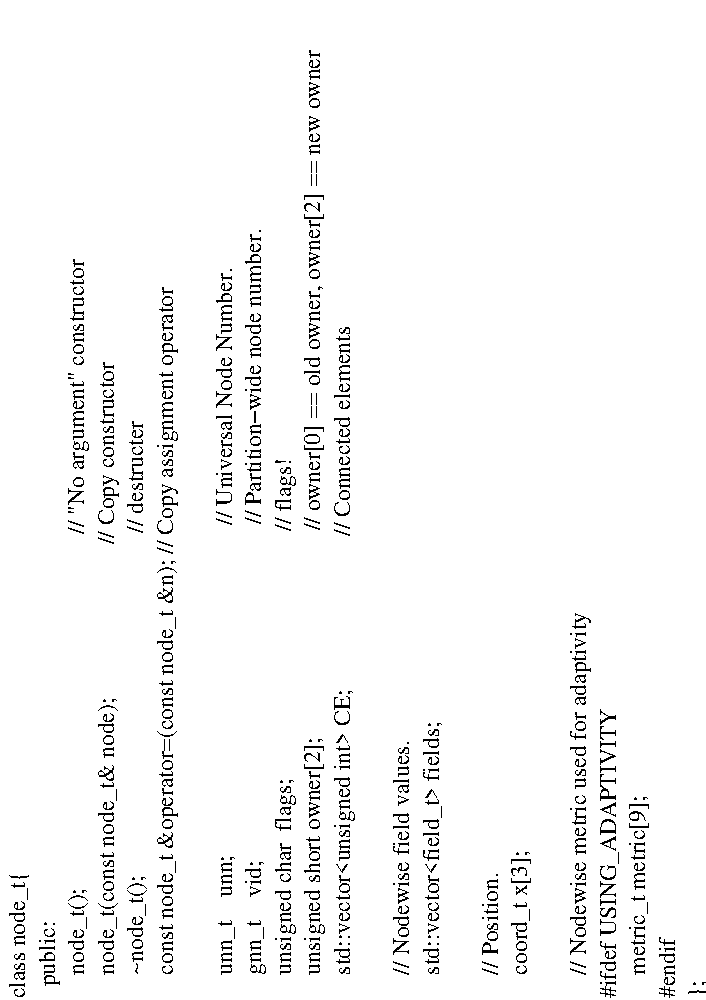
\includegraphics[height=140mm, angle=-90]{images/node_class}
\caption{C++ node class}
\end{figure} 

\begin{figure}[h]\label{fig:element_class}
\centering
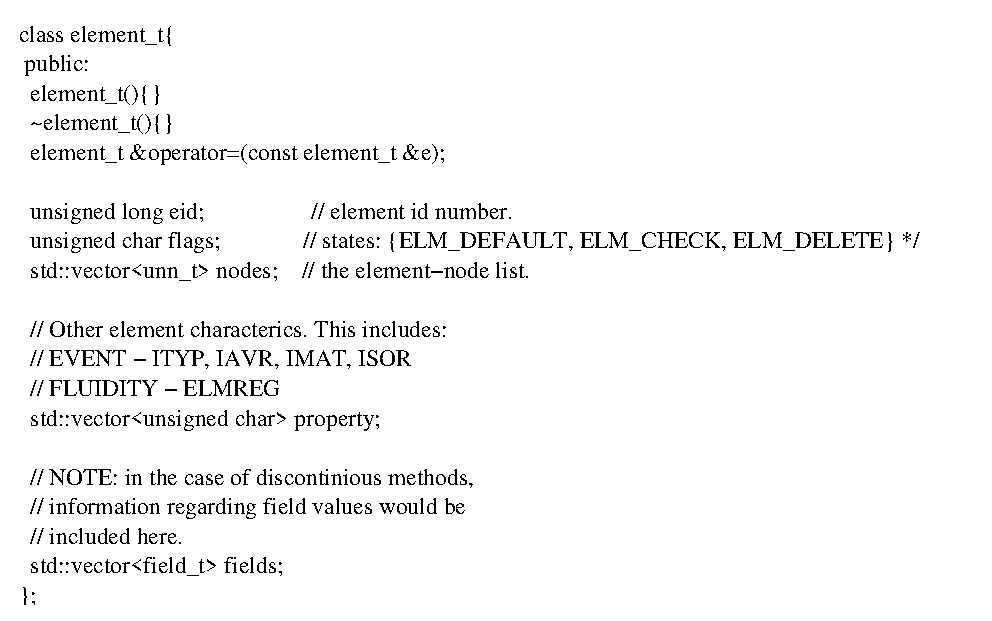
\includegraphics[height=140mm, angle=-90]{images/element_class}
\caption{C++ element class}
\end{figure} 

\begin{figure}[h]\label{fig:mesh_class}
\centering
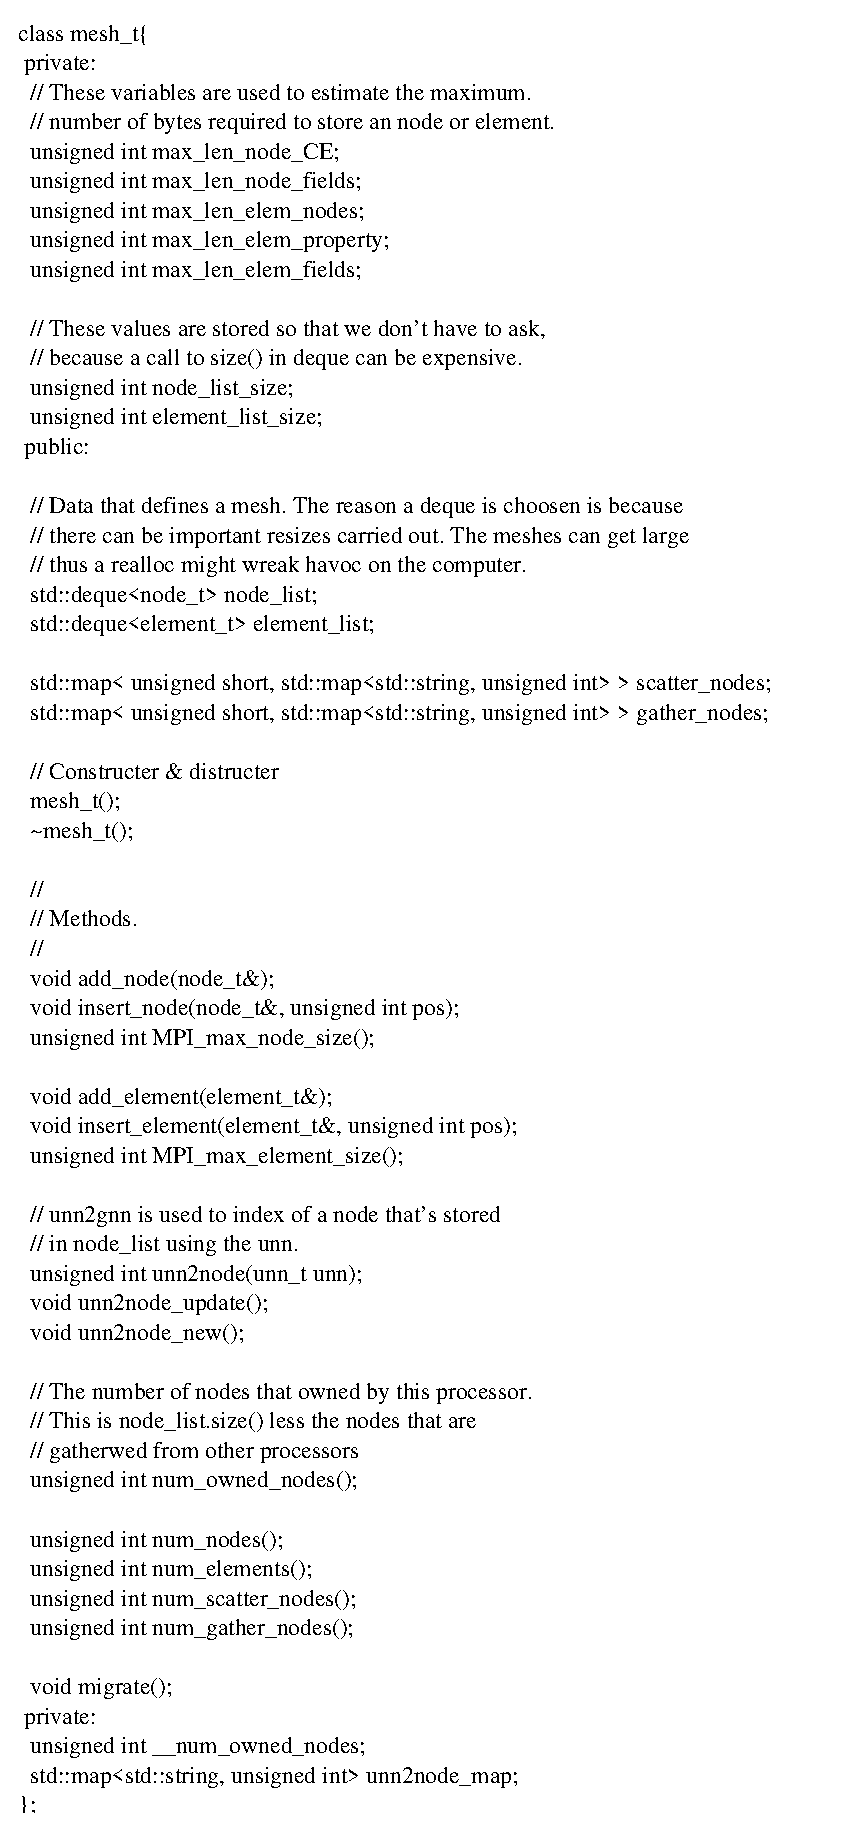
\includegraphics[width=210mm, angle=-90]{images/mesh_class}
\caption{C++ mesh class}
\end{figure} 

\section{Users Manual}

In order that this library can be used with a Fortran application such
as FLUIDITY or EVENT, a C++ patch must be created for the application.
This can be easily done via a generic script and an extra rule in the
applications Makefile. With the {\it libmigrate} source the script
{\it mkcxxpatch} there is a script
provided to generate the appropriate patch. This script
takes the main Fortran source file as an argument and generates a file
called c++main\_patch.f which should be compiled with the rest of the
application. A simple version of the script is shown in Figure~\ref{fig:mkcxxpatch}.
\begin{figure}[h]\label{fig:mkcxxpatch}
\centering
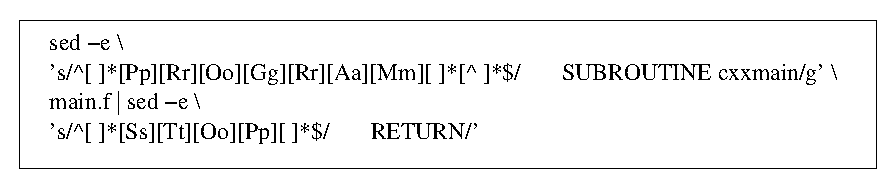
\includegraphics[height=140mm, angle=-90]{images/mkcxxpatch}
\caption{Example script that generates a C++ patch from a Fortran 77
file which contains a main routine}
\end{figure} 
%A simple version of the script is shown below:
%sed -e $\backslash$ \\
%'s/\textasciicircum [ ]*[Pp][Rr][Oo][Gg][Rr][Aa][Mm][
%]*[\textasciicircum ]*\$/~~~~~~SUBROUTINE cxxmain/g'$\backslash$\\
%mainfl.f \textbar sed -e $\backslash$ \\
%'s/\textasciicircum[ ]*[Ss][Tt][Oo][Pp][ ]*\$/~~~~~~RETURN/' \textgreater c++main\_patch.f\\

When the {\it mesh} class from {\it libmigrate} is being used, then
the migration operation is used by first updating the {\it new owner}
data in the {\it node} class and then calling the {\it mesh} member
function {\it migrate}. Then the operation is to be called from a
Fortran, a specialised C++ function, or {\it wrapper}, must be written
to interface with the Fortran code. The interface proceeds as follows:
\begin{itemize}
\item Fortran calls the interface subroutine
\item the wrapper maps the arguments that were passed in to {\it
libmigrate}'s classes
\item migration of nodes is performed
\item the new mesh is passed back to the calling routine with a
specified mapping.
\end{itemize}

One specialised wrapper has already been written for FLUIDITY. To use,
FLUIDITY is linked using {\it mpiCC} and with the additional linking
flags {\it -lfor -lUfor -lmigrate -lm -lstdc++}. The interface for the
migration subroutine is shown in Figure~\ref{fig:fluidity_migrate_interface}.

\section{Future Work/Conclusion}
\begin{itemize}
\item Add support for higher order node adjacency
\item Develop a complementary library for graph partitioning and load
balancing
\item Develop a complementary library for mesh adaptivity
\end{itemize}

\section{Acknowledgements}
Many thanks to Mr Adrian P. Umpleby for his useful comments and
guidance in the development of the algorithm used for the migration.

\bibliographystyle{plain}
\bibliography{migrate}

\end{document}






















